\documentclass[11pt, twoside]{article}

\usepackage{graphicx}
\usepackage{amsmath}
\usepackage{amssymb}
\usepackage{verbatim} 
\usepackage{subfigure}
\usepackage{amsfonts}
\usepackage{hyperref}
%\usepackage{tikz}



\RequirePackage[usenames,dvipsnames]{color}
\RequirePackage{fancyhdr}
\RequirePackage{graphicx}

% to include C++ code:
\usepackage{listings}
\usepackage{xcolor}
\lstset { %
	language=C++,
	backgroundcolor=\color{black!5}, % set backgroundcolor
	basicstyle=\footnotesize,% basic font setting
}

%------------------- settings margini ----
\setlength{\oddsidemargin}{-15pt}
\setlength{\evensidemargin}{-15pt}
\setlength{\marginparwidth}{0pt}
\setlength{\textwidth}{500pt}
\setlength{\topmargin}{-40pt}
\setlength{\textheight}{650pt}

\newcommand{\cambiaFont}[2]{{\fontencoding{T1}\fontfamily{#1}%
		\selectfont#2}}

%-------- pacchetti base------------------
\usepackage[english]{babel}
\usepackage{euscript}
\usepackage[utf8]{inputenc}
%------ per i diagrammi commutativi: 
\usepackage{pictexwd,dcpic}
\usepackage[all]{xy}

%---- fancyheader and footer 
%\fancyhead{} % clear all fields
%\fancyhead[LE]{\thepage~~~~\textrm{asdf}~~\textit{asdffda}}
%\fancyhead[RO]{ {\sf Ricerca di Crittografia}, ~~~~\thepage}
\fancyfoot{}
\fancyfoot[RO]{ {\small  MPHYG002: Research Computing with C++, ~\thepage}}
\fancyfoot[LE]{ {\small \thepage,~ Coursework 2 }}
\renewcommand{\headrulewidth}{0.0pt}



\begin{document}

% %--------- pagenumbering ------------
\setcounter{page}{1}
\pagestyle{fancy} 
% %----------------------------------------



% ----  TITLE DATE ---- 
~\vspace{-2cm} 
\begin{center}  	
	
	\hrule
	
	\vspace{0.5cm} 
	\color{Black} MPHYG002: Research Computing with C++ \color{Black}
	\vspace{0.5cm} \\
	\cambiaFont{ppl}{ \color{MidnightBlue} $\bullet$ \color{MidnightBlue} ~{\Large Coursework 2 - Conway's Game of Life } ~ \color{MidnightBlue}$\bullet$\color{black}} 
	\vspace{0.3cm} \\
	Sebastiano Ferraris  ~ SN: 14108168 ~  s.ferraris@ucl.ac.uk ~ \today 
	\vspace{0.5cm} 
	\hrule
	
\end{center}

\vspace{0.1in}


%--- autore



%------------ indice eventuale:
 %\tableofcontents
%____________________________


\begin{center}
	\color{MidnightBlue} {\Large Introducing the Game }\color{Black} 
\end{center}

\noindent
\href{https://en.wikipedia.org/wiki/Conway%27s_Game_of_Life}{Conway's Game of Life} is a deterministic evolutionary discrete event dynamical system played on an infinite 2-dimensional grid.
At each position of the gird there is a cell, that can be in two states: \emph{alive} 1, or \emph{dead} 0.
The state of cell $C$ at time $t$, indicated with $\text{state}_t(C)$ evolves over a discrete time according to its degree. The degree of a cell, $\text{deg}_t(C)$ is the number of alive cells into its eight neigbours, and the evolution model from the state $t$ to the state $t+1$ happens according to the following rules, called update rule, applied simultaneously for all the cells in the grid for a given time-state:
\begin{enumerate}
	\item $\text{state}_t(C) = 1$ and $\text{deg}_t(C)<2$ then $\text{state}_{t+1}(C) = 0$.
	\item $\text{state}_t(C) = 1$ and $2 \leq\text{deg}_t(C) \leq 3$ then $\text{state}_{t+1}(C) = 1$.
	\item $\text{state}_t(C) = 1$ and $\text{deg}_t(C)>3$ then $\text{state}_{t+1}(C) = 0$.
	\item $\text{state}_t(C) = 0$ and $\text{deg}_t(C)=3$ then $\text{state}_{t+1}(C) = 1$.
\end{enumerate}
The initial state is called \emph{seed}, and it completely determines the subsequent steps of the game.

\begin{figure}[htbp]
	\centering
	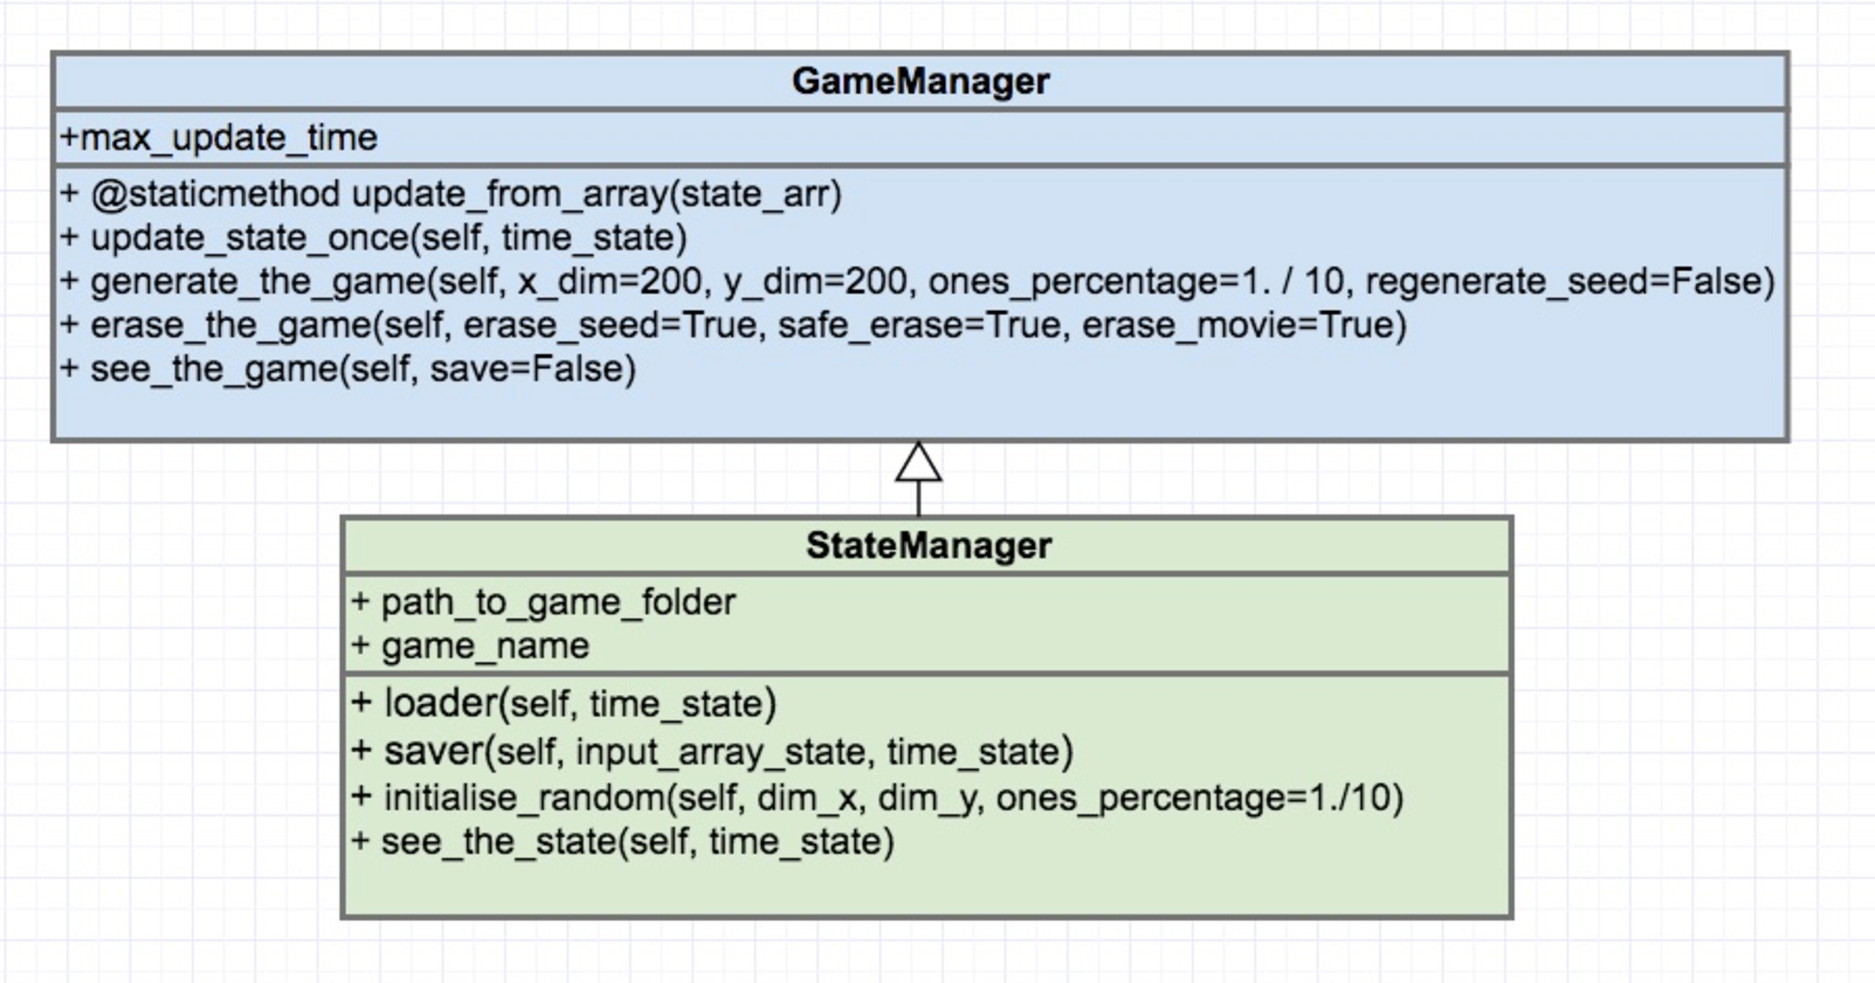
\includegraphics[scale=0.45]{figures/uml_py.pdf}
	\caption{UML diagram representing the structure proposed for the StateManager and the GameManager classes implemented in python.}
	\label{fig:uml_py}
\end{figure}


\begin{center}
	\color{MidnightBlue} {\Large Part 1: Serial Solution }\color{Black} 
\end{center}

\noindent
In the simple implementation here proposed, a \emph{state} is represented by a \emph{.txt} file that contains a binary matrix whose zeros represents the dead cells and ones represents the living cells. A \emph{game}, in the perspective here proposed, is a sequence of $.txt$ file where in the filename appears the name of the game, shared for each state, and an integer time parameter, starting from $0$ for the seed. Two states with consecutive indexes are related to each others by the update rule, and the finite grid is considered with a toroidal equivalence relation on the edges, to make it if not periodic, at least infinite.
Given the need of plotting computing statistics for computational comparisons purposes and of obtaining an animation of a game (see the README.md on github \href{https://github.com/SebastianoF/game_of_life}{repository}), I opted for wrapping the C++ code inside python with boost::python, and to call the shared object (.so) generated with the C++ compiler as libraries inside python code. \\

\noindent
\color{MidnightBlue} {\Large Design and code structure }\color{Black}  \\
The object oriented structure is driven by the definition of state and game. To reduce computational costs and the length of the code, there is no class implemented for a state or a game, being structured .txt files. The classes are implemented for the operations between states, as well as to create random seeds, visualize states and games.

\begin{figure}[htbp]
	\centering
	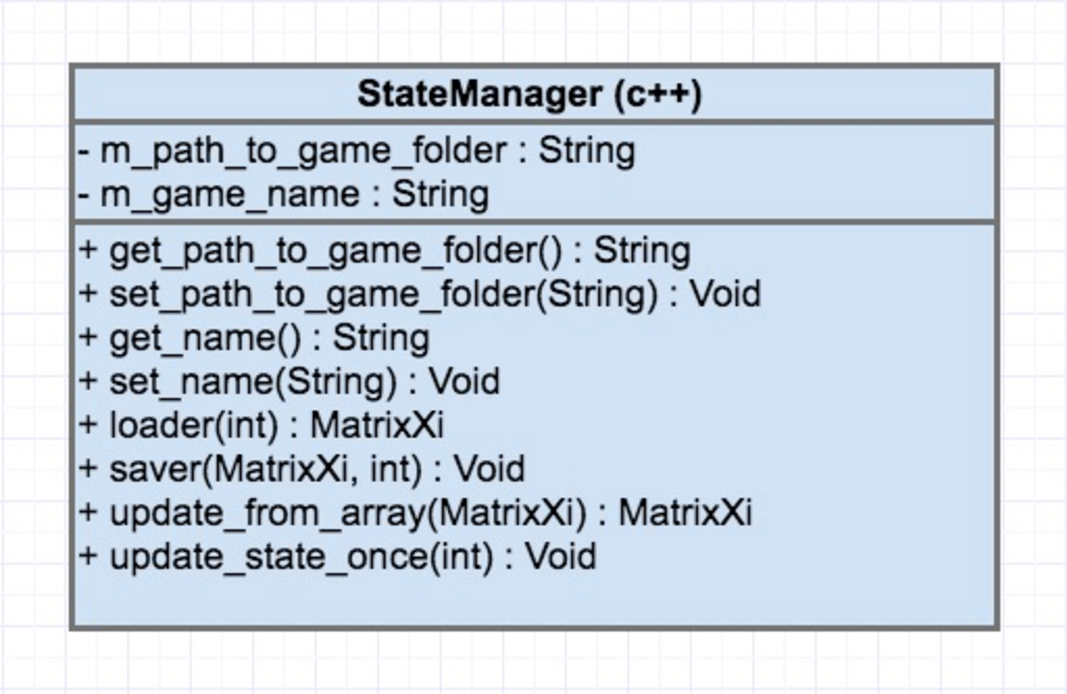
\includegraphics[scale=0.45]{figures/uml_cpp.pdf}
	\caption{UML diagram representing the structure proposed for the StateManager and the GameManager classes implemented in C++.}
	\label{fig:uml_cpp}
\end{figure}

\noindent
The folder structure is organized as follows:
\begin{itemize}
	\item[{\bf examples}] - contains some hello-world style examples and some code to create games of life, from random seeds and from seeds created ad hoc.
	\item[{\bf report}] contains this report and the figures produced with statistical methods.
	\item[{\bf src}] is divided into:
	\begin{itemize}
		\item[{\bf core}] where the core libraries having the classes, in python and C++ are stored.
		\item[{\bf utils}] where auxiliaries functions and visualisation methods are stored.
	\end{itemize}
	\item[{\bf stats}] contains the methods that produced the statistical results.
	\item[{\bf test}] contains the tests, performed with the library Nosetest. The C++ code is tested here as well, in its main functions.
\end{itemize}

\begin{center}
	\color{MidnightBlue} {\Large Part 2: Parallel computation - OpenMP }\color{Black} 
\end{center}

A simple code with a parallelised version of the C++ StateManager is implemented and its performance is compared with the non parallel version. The main for-cycle in the code, for loading the \emph{.txt} files and for update the states are parallelized with a simple OMP environment
\begin{verbatim}
#pragma omp parallel for
\end{verbatim}
If OpenMP is not available to the compiler then the parallelisation is ignored, thanks to the following workaround proposed in the code:
\begin{verbatim}
#if defined(ENABLE_OPENMP)
  #include <omp.h>
#else
  typedef int omp_int_t;
  inline omp_int_t omp_get_thread_num() { return 0;}
  inline omp_int_t omp_get_max_threads() { return 1;}
#endif
\end{verbatim}


\begin{center}
	\color{MidnightBlue} {\Large Part 3: Remote computation}\color{Black} 
\end{center}
\noindent
To run a python script of the project on a cluster (for example \emph{play\textunderscore a\textunderscore game\textunderscore cpp\textunderscore omp.py} ) we propose to copy the code on the cluster with the command \emph{scp}, and then to type
\begin{verbatim}
nohup ./MasterRun.sh &
\end{verbatim}
This command run a script that calls the \emph{qsub} as in the following code:
\begin{verbatim}
qsub -l h_rt=49:00:00 -l tmem=15G -l h_vmem=15G  -cwd  -v FOLDER=path-to-data-folder
path-to-script-folder/play.sh;
\end{verbatim}
In this way the \emph{qsub} command has its own script that includes the chosen parameters and the path to the data folder in the cluster.
The bash script \emph{play.sh} has finally the command for the cluster with the python code:
\begin{verbatim}
#!/bin/bash
/home/path_to_python/python/bin/python2.7 path-to-examples/play_a_game_cpp_omp.py ${FOLDER}
\end{verbatim}
And to include the path with the data as an input parameter, we have to add the following line in the file \emph{play\textunderscore a\textunderscore game\textunderscore cpp\textunderscore omp.py}
\begin{verbatim}
path_to_game_folder = sys.argv[1]
\end{verbatim}




\begin{figure}
	\centering
	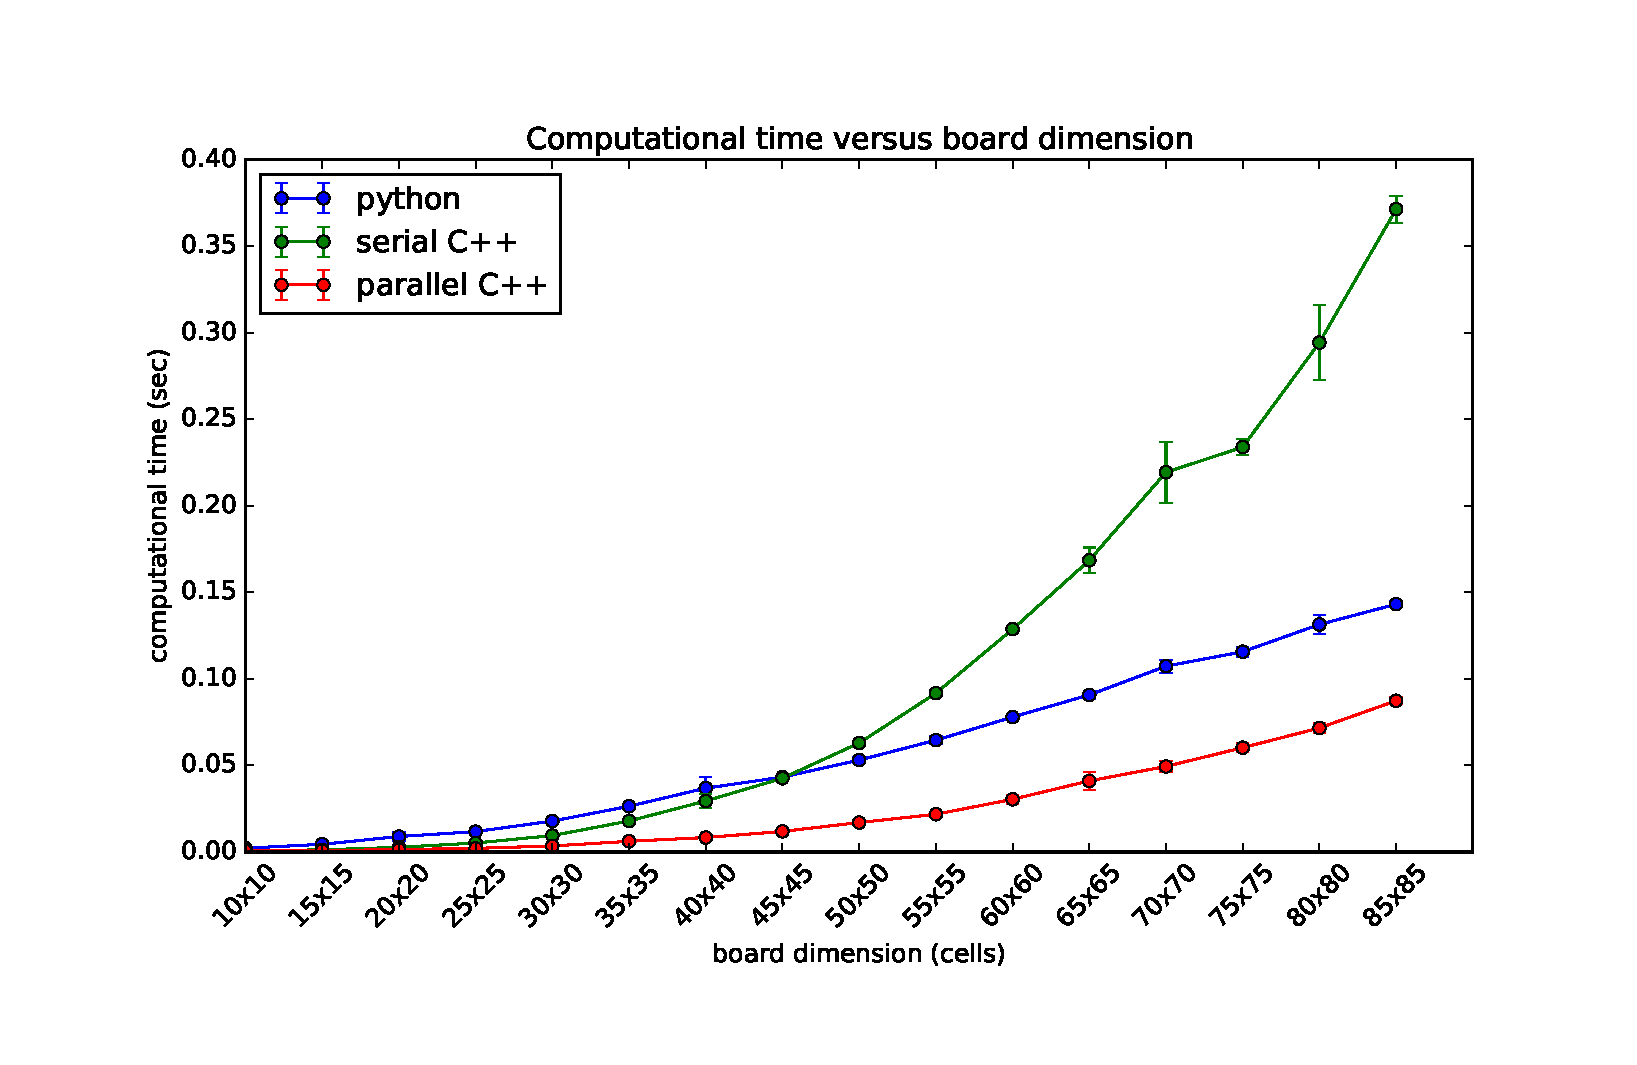
\includegraphics[scale=0.55]{figures/figure_1.pdf}
	\caption{Comparison in computational time for an increasing grid. The computational time is the one computed to run a full game, and the mean is computed for a random sample of $10$ initial seeds. Each game is computed for $30$ time points.}
	\label{fig:graph}
\end{figure}




\begin{center}
	\color{MidnightBlue} {\Large Conclusions}\color{Black} 
\end{center}

\noindent
In an experiment, we compared the computational time of a pure python implementation, with the one implemented with C++ and the one parallelised with OpenMP. Results show that the serial C++ version is slower than the python implementation for board larger than $45\times 45$, while the parallelised is the fastest implementation for any of the chosen board dimension.
The discrepancy between the python and the serial C++ can be explained by the fact that the \emph{loader} method to store each state in .txt in a numpy.ndarray or in an Eigen::MatrixXi is optimised for python, while it is not for the case of the serial C++.\\

\noindent
A fair computational complexity analysis that is not biased by this problem, needs to have methods in C++ that can have numpy.ndarray as input, or vice versa, methods in python that can work with Eigen C++ library matrix as input.
An option is given by the library eigency of Cython, that provides an interface between these two data structure. And in general a comparison between Cython version of game of life an the optimised C++ library can be a good option for future work.


\vspace{1cm}
\noindent
Please see the link include in the README.md on the github \href{https://github.com/SebastianoF/game_of_life}{repository} for references.
\end{document}





